\documentclass[twoside]{book}

% Packages required by doxygen
\usepackage{fixltx2e}
\usepackage{calc}
\usepackage{doxygen}
\usepackage[export]{adjustbox} % also loads graphicx
\usepackage{graphicx}
\usepackage[utf8]{inputenc}
\usepackage{makeidx}
\usepackage{multicol}
\usepackage{multirow}
\PassOptionsToPackage{warn}{textcomp}
\usepackage{textcomp}
\usepackage[nointegrals]{wasysym}
\usepackage[table]{xcolor}

% Font selection
\usepackage[T1]{fontenc}
\usepackage[scaled=.90]{helvet}
\usepackage{courier}
\usepackage{amssymb}
\usepackage{sectsty}
\renewcommand{\familydefault}{\sfdefault}
\allsectionsfont{%
  \fontseries{bc}\selectfont%
  \color{darkgray}%
}
\renewcommand{\DoxyLabelFont}{%
  \fontseries{bc}\selectfont%
  \color{darkgray}%
}
\newcommand{\+}{\discretionary{\mbox{\scriptsize$\hookleftarrow$}}{}{}}

% Page & text layout
\usepackage{geometry}
\geometry{%
  a4paper,%
  top=2.5cm,%
  bottom=2.5cm,%
  left=2.5cm,%
  right=2.5cm%
}
\tolerance=750
\hfuzz=15pt
\hbadness=750
\setlength{\emergencystretch}{15pt}
\setlength{\parindent}{0cm}
\setlength{\parskip}{3ex plus 2ex minus 2ex}
\makeatletter
\renewcommand{\paragraph}{%
  \@startsection{paragraph}{4}{0ex}{-1.0ex}{1.0ex}{%
    \normalfont\normalsize\bfseries\SS@parafont%
  }%
}
\renewcommand{\subparagraph}{%
  \@startsection{subparagraph}{5}{0ex}{-1.0ex}{1.0ex}{%
    \normalfont\normalsize\bfseries\SS@subparafont%
  }%
}
\makeatother

% Headers & footers
\usepackage{fancyhdr}
\pagestyle{fancyplain}
\fancyhead[LE]{\fancyplain{}{\bfseries\thepage}}
\fancyhead[CE]{\fancyplain{}{}}
\fancyhead[RE]{\fancyplain{}{\bfseries\leftmark}}
\fancyhead[LO]{\fancyplain{}{\bfseries\rightmark}}
\fancyhead[CO]{\fancyplain{}{}}
\fancyhead[RO]{\fancyplain{}{\bfseries\thepage}}
\fancyfoot[LE]{\fancyplain{}{}}
\fancyfoot[CE]{\fancyplain{}{}}
\fancyfoot[RE]{\fancyplain{}{\bfseries\scriptsize Generated by Doxygen }}
\fancyfoot[LO]{\fancyplain{}{\bfseries\scriptsize Generated by Doxygen }}
\fancyfoot[CO]{\fancyplain{}{}}
\fancyfoot[RO]{\fancyplain{}{}}
\renewcommand{\footrulewidth}{0.4pt}
\renewcommand{\chaptermark}[1]{%
  \markboth{#1}{}%
}
\renewcommand{\sectionmark}[1]{%
  \markright{\thesection\ #1}%
}

% Indices & bibliography
\usepackage{natbib}
\usepackage[titles]{tocloft}
\setcounter{tocdepth}{3}
\setcounter{secnumdepth}{5}
\makeindex

% Hyperlinks (required, but should be loaded last)
\usepackage{ifpdf}
\ifpdf
  \usepackage[pdftex,pagebackref=true]{hyperref}
\else
  \usepackage[ps2pdf,pagebackref=true]{hyperref}
\fi
\hypersetup{%
  colorlinks=true,%
  linkcolor=blue,%
  citecolor=blue,%
  unicode%
}

% Custom commands
\newcommand{\clearemptydoublepage}{%
  \newpage{\pagestyle{empty}\cleardoublepage}%
}

\usepackage{caption}
\captionsetup{labelsep=space,justification=centering,font={bf},singlelinecheck=off,skip=4pt,position=top}

%===== C O N T E N T S =====

\begin{document}

% Titlepage & ToC
\hypersetup{pageanchor=false,
             bookmarksnumbered=true,
             pdfencoding=unicode
            }
\pagenumbering{alph}
\begin{titlepage}
\vspace*{7cm}
\begin{center}%
{\Large Trajektoria }\\
\vspace*{1cm}
{\large Generated by Doxygen 1.8.14}\\
\end{center}
\end{titlepage}
\clearemptydoublepage
\pagenumbering{roman}
\tableofcontents
\clearemptydoublepage
\pagenumbering{arabic}
\hypersetup{pageanchor=true}

%--- Begin generated contents ---
\chapter{Hierarchical Index}
\section{Class Hierarchy}
This inheritance list is sorted roughly, but not completely, alphabetically\+:\begin{DoxyCompactList}
\item \contentsline{section}{Punkt}{\pageref{struct_punkt}}{}
\item Q\+Dialog\begin{DoxyCompactList}
\item \contentsline{section}{autor}{\pageref{classautor}}{}
\item \contentsline{section}{pokaz\+Traj}{\pageref{classpokaz_traj}}{}
\item \contentsline{section}{Save\+Dialog}{\pageref{class_save_dialog}}{}
\item \contentsline{section}{statystyki}{\pageref{classstatystyki}}{}
\end{DoxyCompactList}
\item Q\+Main\+Window\begin{DoxyCompactList}
\item \contentsline{section}{Main\+Window}{\pageref{class_main_window}}{}
\end{DoxyCompactList}
\end{DoxyCompactList}

\chapter{Class Index}
\section{Class List}
Here are the classes, structs, unions and interfaces with brief descriptions\+:\begin{DoxyCompactList}
\item\contentsline{section}{\mbox{\hyperlink{classautor}{autor}} }{\pageref{classautor}}{}
\item\contentsline{section}{\mbox{\hyperlink{class_main_window}{Main\+Window}} }{\pageref{class_main_window}}{}
\item\contentsline{section}{\mbox{\hyperlink{classpokaz_traj}{pokaz\+Traj}} }{\pageref{classpokaz_traj}}{}
\item\contentsline{section}{\mbox{\hyperlink{struct_punkt}{Punkt}} }{\pageref{struct_punkt}}{}
\item\contentsline{section}{\mbox{\hyperlink{class_save_dialog}{Save\+Dialog}} }{\pageref{class_save_dialog}}{}
\item\contentsline{section}{\mbox{\hyperlink{classstatystyki}{statystyki}} }{\pageref{classstatystyki}}{}
\end{DoxyCompactList}

\chapter{Class Documentation}
\hypertarget{classautor}{}\section{autor Class Reference}
\label{classautor}\index{autor@{autor}}
Inheritance diagram for autor\+:\begin{figure}[H]
\begin{center}
\leavevmode
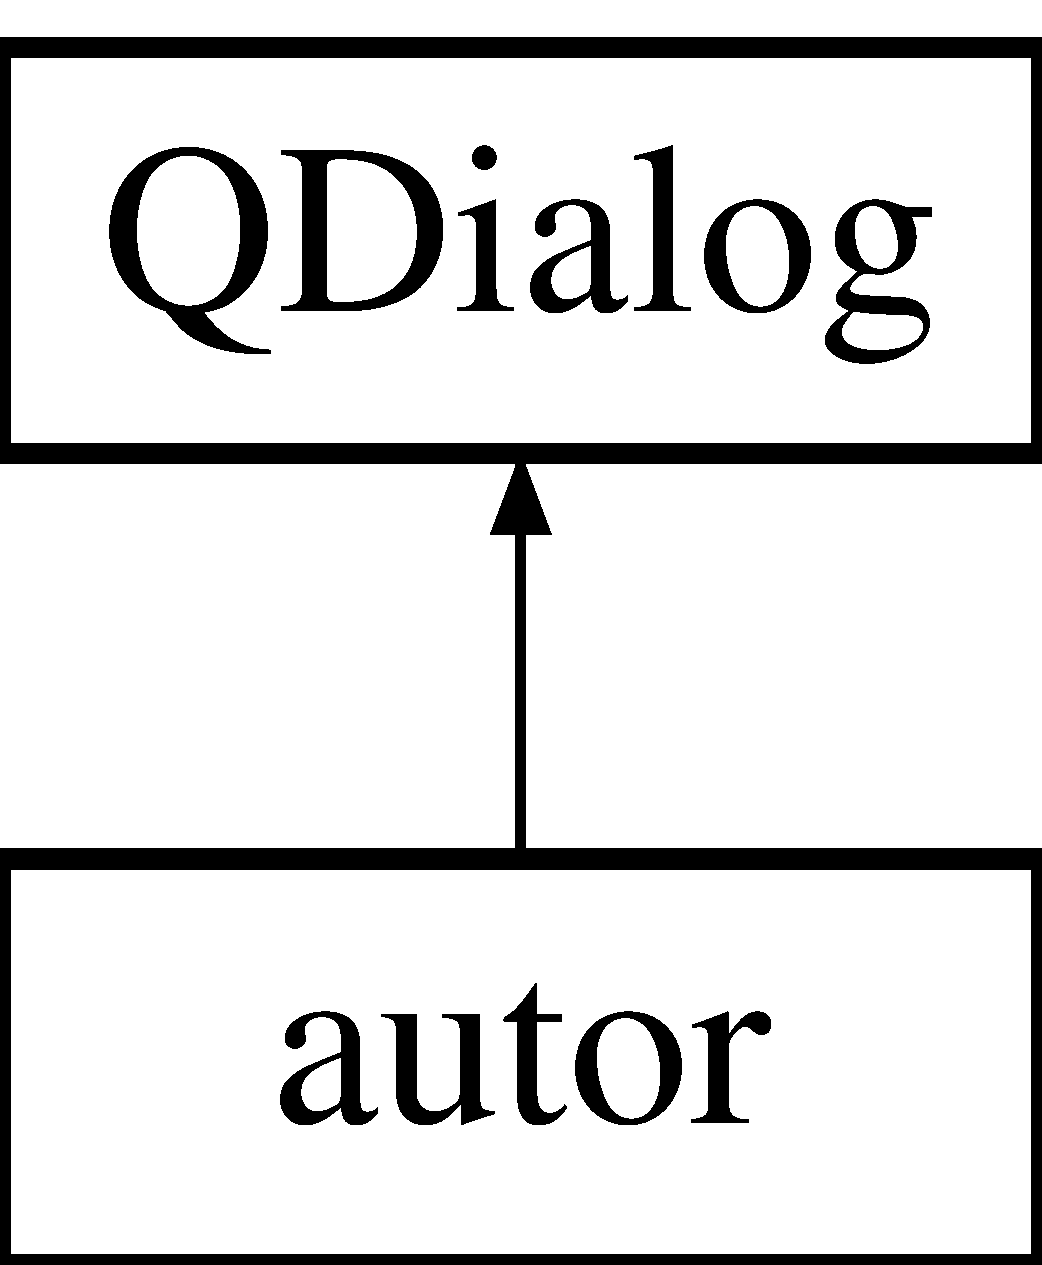
\includegraphics[height=2.000000cm]{classautor}
\end{center}
\end{figure}
\subsection*{Public Member Functions}
\begin{DoxyCompactItemize}
\item 
\mbox{\Hypertarget{classautor_a83ce50c391a01b97decc7a0e9651eb80}\label{classautor_a83ce50c391a01b97decc7a0e9651eb80}} 
{\bfseries autor} (Q\+Widget $\ast$parent=0)
\end{DoxyCompactItemize}


The documentation for this class was generated from the following files\+:\begin{DoxyCompactItemize}
\item 
autor.\+h\item 
autor.\+cpp\end{DoxyCompactItemize}

\hypertarget{class_main_window}{}\section{Main\+Window Class Reference}
\label{class_main_window}\index{Main\+Window@{Main\+Window}}
Inheritance diagram for Main\+Window\+:\begin{figure}[H]
\begin{center}
\leavevmode
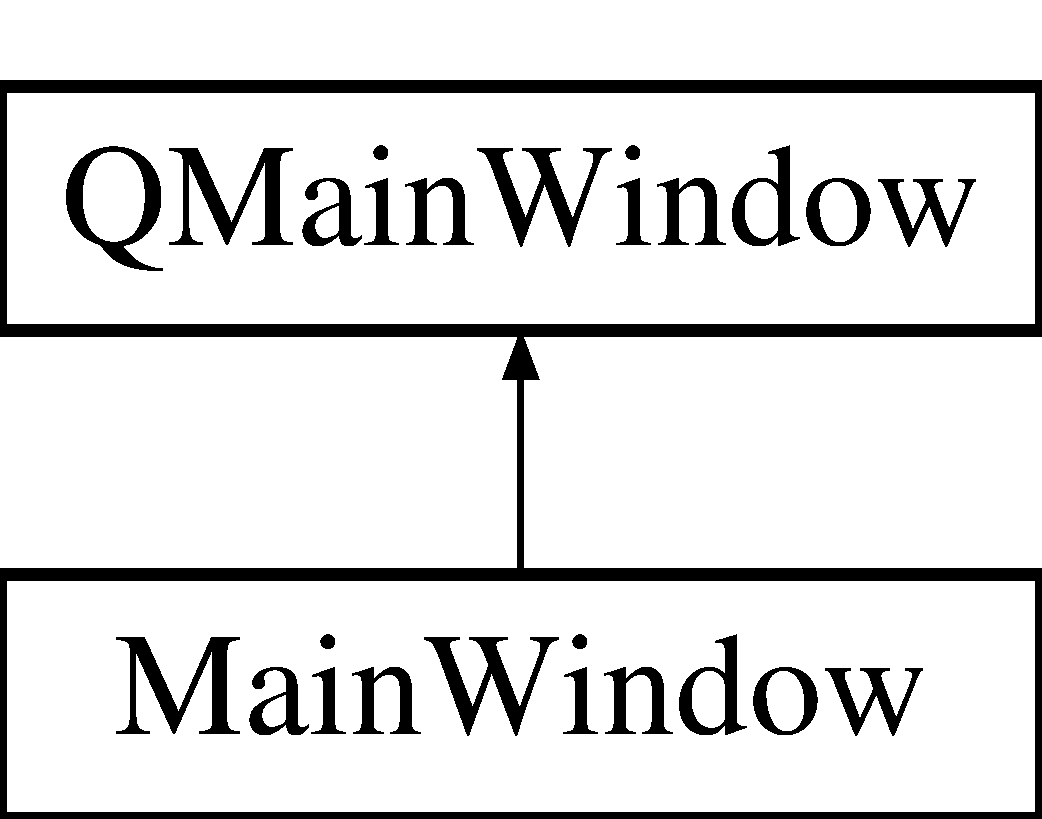
\includegraphics[height=2.000000cm]{class_main_window}
\end{center}
\end{figure}
\subsection*{Public Slots}
\begin{DoxyCompactItemize}
\item 
\mbox{\Hypertarget{class_main_window_af3c0acb6430798883d9df9dadea3b725}\label{class_main_window_af3c0acb6430798883d9df9dadea3b725}} 
void {\bfseries zapisz\+Plik} (Q\+String nazwa)
\end{DoxyCompactItemize}
\subsection*{Signals}
\begin{DoxyCompactItemize}
\item 
\mbox{\Hypertarget{class_main_window_ae47c4ed1673da6c67f1bf071109f2fbd}\label{class_main_window_ae47c4ed1673da6c67f1bf071109f2fbd}} 
void {\bfseries przeslij\+\_\+liste} (\mbox{\hyperlink{struct_punkt}{Punkt}} $\ast$g)
\end{DoxyCompactItemize}
\subsection*{Public Member Functions}
\begin{DoxyCompactItemize}
\item 
\mbox{\Hypertarget{class_main_window_a8b244be8b7b7db1b08de2a2acb9409db}\label{class_main_window_a8b244be8b7b7db1b08de2a2acb9409db}} 
{\bfseries Main\+Window} (Q\+Widget $\ast$parent=0)
\end{DoxyCompactItemize}
\subsection*{Public Attributes}
\begin{DoxyCompactItemize}
\item 
\mbox{\Hypertarget{class_main_window_ae07483988be03b22941a090dc36836df}\label{class_main_window_ae07483988be03b22941a090dc36836df}} 
double {\bfseries G}
\item 
\mbox{\Hypertarget{class_main_window_afe8a5e23f01e4779ad2bf9dddd470351}\label{class_main_window_afe8a5e23f01e4779ad2bf9dddd470351}} 
double {\bfseries Cd}
\item 
\mbox{\Hypertarget{class_main_window_a3e24497d6e558c83fd2b13d13aeb8db1}\label{class_main_window_a3e24497d6e558c83fd2b13d13aeb8db1}} 
double {\bfseries A}
\item 
\mbox{\Hypertarget{class_main_window_a555e4c65f17f825ed8790bb592cafed6}\label{class_main_window_a555e4c65f17f825ed8790bb592cafed6}} 
double {\bfseries Ro}
\item 
\mbox{\Hypertarget{class_main_window_a59ffdff998bf720fca8709eec9035b26}\label{class_main_window_a59ffdff998bf720fca8709eec9035b26}} 
double {\bfseries Masa}
\item 
\mbox{\Hypertarget{class_main_window_ab319253eb1520a69c4d8b435f4c54330}\label{class_main_window_ab319253eb1520a69c4d8b435f4c54330}} 
double {\bfseries Skok}
\item 
\mbox{\Hypertarget{class_main_window_a8cdea7d6a643c5fd2cfdcccc7b07ae28}\label{class_main_window_a8cdea7d6a643c5fd2cfdcccc7b07ae28}} 
double {\bfseries S} \mbox{[}6\mbox{]}
\item 
\mbox{\Hypertarget{class_main_window_aff1acdcf582000aa1f7e764ba590aa9d}\label{class_main_window_aff1acdcf582000aa1f7e764ba590aa9d}} 
double {\bfseries W} \mbox{[}4\mbox{]}
\item 
\mbox{\Hypertarget{class_main_window_ae6e89bf5abd465f0ca42d42e76ce4ec2}\label{class_main_window_ae6e89bf5abd465f0ca42d42e76ce4ec2}} 
double {\bfseries O} \mbox{[}3\mbox{]}
\item 
\mbox{\Hypertarget{class_main_window_abf84e162db3023e0da8a062681906ace}\label{class_main_window_abf84e162db3023e0da8a062681906ace}} 
double {\bfseries Ob} \mbox{[}5\mbox{]}\mbox{[}3\mbox{]}
\item 
\mbox{\Hypertarget{class_main_window_ad62f37d4092d5c8f2fcb64adf9eab349}\label{class_main_window_ad62f37d4092d5c8f2fcb64adf9eab349}} 
string {\bfseries nazwa\+\_\+pliku}
\item 
\mbox{\Hypertarget{class_main_window_a728146f11fd01f59fed7e9af021a61bd}\label{class_main_window_a728146f11fd01f59fed7e9af021a61bd}} 
bool {\bfseries atmosfera}
\item 
\mbox{\Hypertarget{class_main_window_a353964a574b9af9328cf43567da94fd2}\label{class_main_window_a353964a574b9af9328cf43567da94fd2}} 
int {\bfseries indx}
\end{DoxyCompactItemize}


The documentation for this class was generated from the following files\+:\begin{DoxyCompactItemize}
\item 
mainwindow.\+h\item 
mainwindow.\+cpp\end{DoxyCompactItemize}

\hypertarget{classpokaz_traj}{}\section{pokaz\+Traj Class Reference}
\label{classpokaz_traj}\index{pokaz\+Traj@{pokaz\+Traj}}
Inheritance diagram for pokaz\+Traj\+:\begin{figure}[H]
\begin{center}
\leavevmode
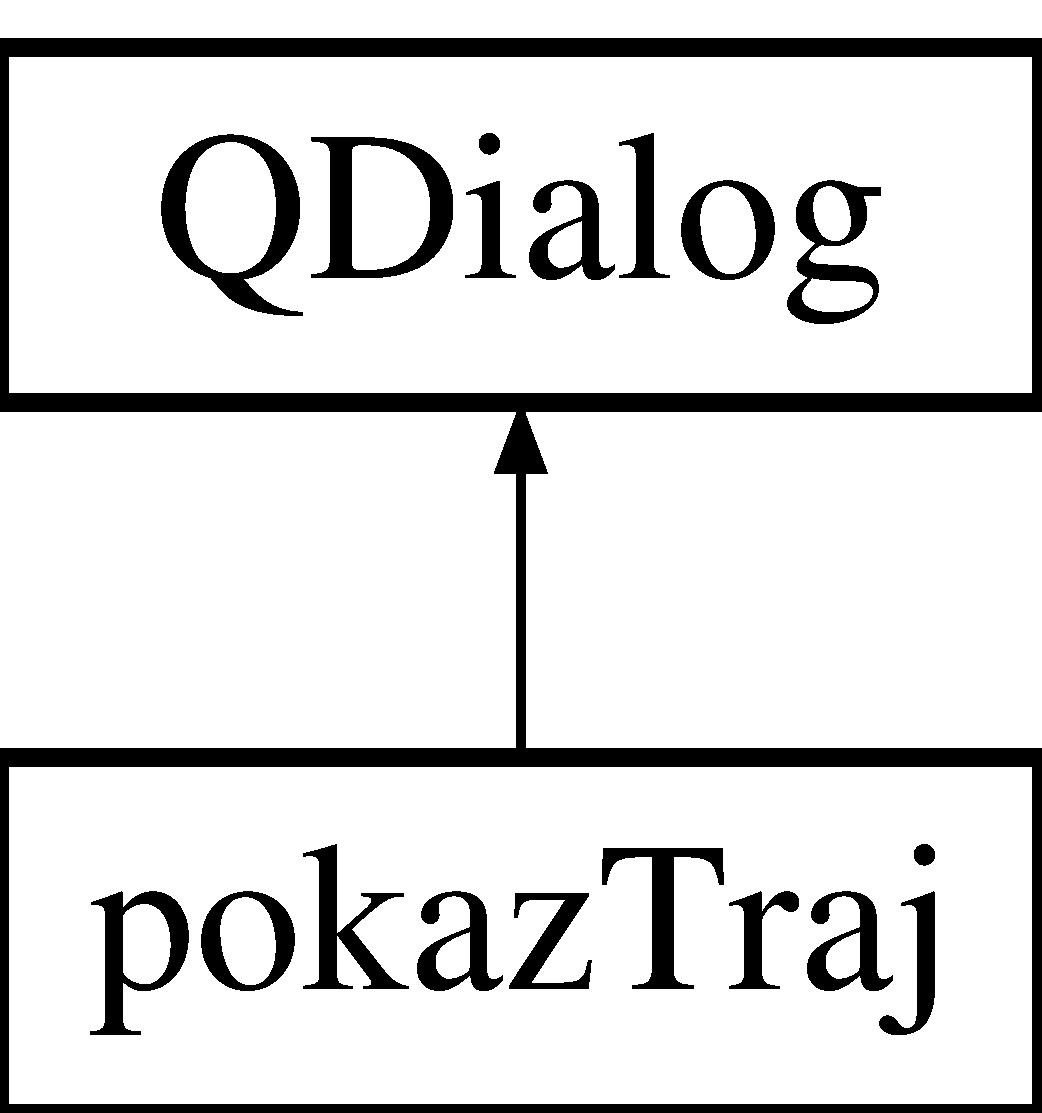
\includegraphics[height=2.000000cm]{classpokaz_traj}
\end{center}
\end{figure}
\subsection*{Public Slots}
\begin{DoxyCompactItemize}
\item 
\mbox{\Hypertarget{classpokaz_traj_a9789951ce1b3f9a34fac38976447c04e}\label{classpokaz_traj_a9789951ce1b3f9a34fac38976447c04e}} 
void {\bfseries zrob\+\_\+trajektorie} (\mbox{\hyperlink{struct_punkt}{Punkt}} $\ast$p)
\end{DoxyCompactItemize}
\subsection*{Public Member Functions}
\begin{DoxyCompactItemize}
\item 
\mbox{\Hypertarget{classpokaz_traj_a30010467d8e1251d3b57762956962349}\label{classpokaz_traj_a30010467d8e1251d3b57762956962349}} 
{\bfseries pokaz\+Traj} (Q\+Widget $\ast$parent=0)
\end{DoxyCompactItemize}


The documentation for this class was generated from the following files\+:\begin{DoxyCompactItemize}
\item 
pokaz\+\_\+traj.\+h\item 
pokaz\+\_\+traj.\+cpp\end{DoxyCompactItemize}

\hypertarget{struct_punkt}{}\section{Punkt Struct Reference}
\label{struct_punkt}\index{Punkt@{Punkt}}
\subsection*{Public Attributes}
\begin{DoxyCompactItemize}
\item 
\mbox{\Hypertarget{struct_punkt_ac01c5fc6681b8faa6cd21060c6b5542c}\label{struct_punkt_ac01c5fc6681b8faa6cd21060c6b5542c}} 
double {\bfseries x}
\item 
\mbox{\Hypertarget{struct_punkt_a1b4dbf2d3c789e8eadea2303186ad1b3}\label{struct_punkt_a1b4dbf2d3c789e8eadea2303186ad1b3}} 
double {\bfseries y}
\item 
\mbox{\Hypertarget{struct_punkt_adc67078d54e8b0d7dec8fce72806aae9}\label{struct_punkt_adc67078d54e8b0d7dec8fce72806aae9}} 
double {\bfseries vx}
\item 
\mbox{\Hypertarget{struct_punkt_a16c4ac61238ed40abf8d70352cd4fd7e}\label{struct_punkt_a16c4ac61238ed40abf8d70352cd4fd7e}} 
double {\bfseries vy}
\item 
\mbox{\Hypertarget{struct_punkt_a8eb1e41a59307a243563e158259c911a}\label{struct_punkt_a8eb1e41a59307a243563e158259c911a}} 
\mbox{\hyperlink{struct_punkt}{Punkt}} $\ast$ {\bfseries n}
\end{DoxyCompactItemize}


The documentation for this struct was generated from the following file\+:\begin{DoxyCompactItemize}
\item 
punkt.\+h\end{DoxyCompactItemize}

\hypertarget{class_save_dialog}{}\section{Save\+Dialog Class Reference}
\label{class_save_dialog}\index{Save\+Dialog@{Save\+Dialog}}
Inheritance diagram for Save\+Dialog\+:\begin{figure}[H]
\begin{center}
\leavevmode
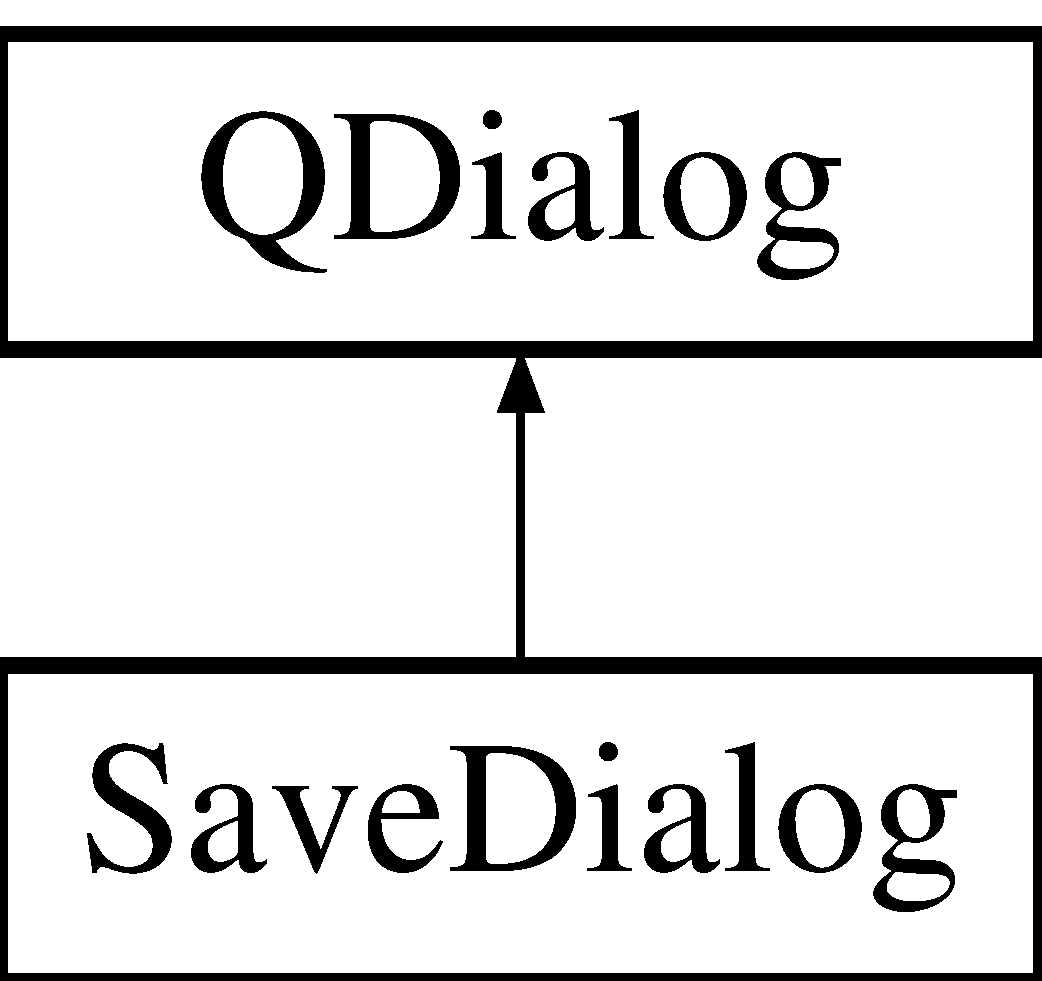
\includegraphics[height=2.000000cm]{class_save_dialog}
\end{center}
\end{figure}
\subsection*{Signals}
\begin{DoxyCompactItemize}
\item 
\mbox{\Hypertarget{class_save_dialog_a6b8f2bf657333aa893275ef4c7f475ee}\label{class_save_dialog_a6b8f2bf657333aa893275ef4c7f475ee}} 
void {\bfseries ustaw\+\_\+tekst} (Q\+String)
\end{DoxyCompactItemize}
\subsection*{Public Member Functions}
\begin{DoxyCompactItemize}
\item 
\mbox{\Hypertarget{class_save_dialog_ac4383e86eb3ff07ce1cd14bc733ea6c7}\label{class_save_dialog_ac4383e86eb3ff07ce1cd14bc733ea6c7}} 
{\bfseries Save\+Dialog} (Q\+Widget $\ast$parent=0)
\end{DoxyCompactItemize}
\subsection*{Public Attributes}
\begin{DoxyCompactItemize}
\item 
\mbox{\Hypertarget{class_save_dialog_a65e839096b4699b16c41be7899743ff4}\label{class_save_dialog_a65e839096b4699b16c41be7899743ff4}} 
Q\+String {\bfseries nazwa\+\_\+pliku}
\end{DoxyCompactItemize}


The documentation for this class was generated from the following files\+:\begin{DoxyCompactItemize}
\item 
savedialog.\+h\item 
savedialog.\+cpp\end{DoxyCompactItemize}

\hypertarget{classstatystyki}{}\section{statystyki Class Reference}
\label{classstatystyki}\index{statystyki@{statystyki}}
Inheritance diagram for statystyki\+:\begin{figure}[H]
\begin{center}
\leavevmode
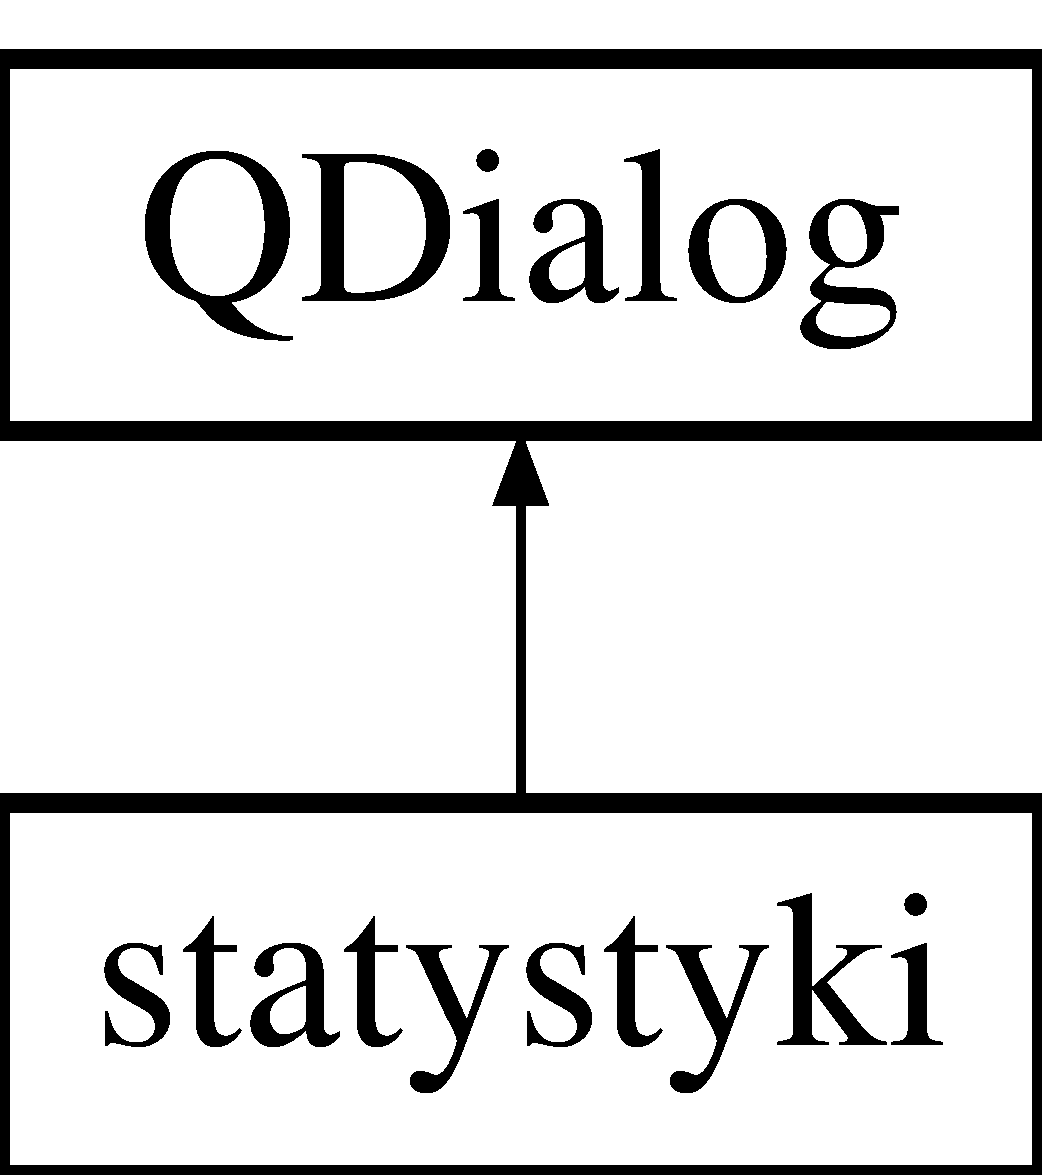
\includegraphics[height=2.000000cm]{classstatystyki}
\end{center}
\end{figure}
\subsection*{Public Slots}
\begin{DoxyCompactItemize}
\item 
\mbox{\Hypertarget{classstatystyki_a9f9e95c6be756519f6abd4b08bbff1f2}\label{classstatystyki_a9f9e95c6be756519f6abd4b08bbff1f2}} 
void {\bfseries przyjmij\+\_\+liste} (\mbox{\hyperlink{struct_punkt}{Punkt}} $\ast$p)
\end{DoxyCompactItemize}
\subsection*{Public Member Functions}
\begin{DoxyCompactItemize}
\item 
\mbox{\Hypertarget{classstatystyki_a93e8666d44ca5614a575a091f4b1eb11}\label{classstatystyki_a93e8666d44ca5614a575a091f4b1eb11}} 
{\bfseries statystyki} (Q\+Widget $\ast$parent=0)
\end{DoxyCompactItemize}


The documentation for this class was generated from the following files\+:\begin{DoxyCompactItemize}
\item 
statystyki.\+h\item 
statystyki.\+cpp\end{DoxyCompactItemize}

%--- End generated contents ---

% Index
\backmatter
\newpage
\phantomsection
\clearemptydoublepage
\addcontentsline{toc}{chapter}{Index}
\printindex

\end{document}
